The purpose of this chapter is to provide a quantifiable assessment of the persistent radio wave energy in the near-Earth space environment due to lightning-generated Whistlers. The morphology of LEP (time evolution, spatial extent at the Earth's surface, and so forth) are primarily determined by the location of wave-particle interactions; additionally, wave-particle interactions with whistlers are hypothesized to be the primary cause of slot-region electron depletions, and the ``impenetrable barrier'' below L $\sim$ 2.

Lightning-generated whistlers are sporadic, and exist alongside a multitude of radio wave activity, such as VLF chorus and plasmaspheric hiss, making a correlated \emph{in-situ} measurement challenging. Within this chapter we simulate the relative VLF energy (L-shell, latitude, longitude) in the near-Earth space environment, in volumetric units [J/$m^3$], as a means of assessing their relative contribution to the persistent radio spectrum.

%\section{Overview of Previous Work}

\section{Methodology}
Our simulation is divided into two portions: First, a simulation of persistent VLF energy due to a single flash originating at a fixed latitude, and second, an integration over a measured lightning dataset, using scaled and shifted ``stencils'' for each flash.

\section{Persistent Energy from a Single Flash}
Figure \ref{fig:power_blockdiagram} shows the steps required to compute the average energy imparted from a single lightning discharge. The resulting stencil has dimensions of L-shell and longitude.
\begin{enumerate}
\item{First we model the sub-ionosphere power spectrum generated from a flash with a known peak current, using the methodology of section \ref{section:input_power}.}
\item{We then propagate the energies through the ionosphere, using the attenuating slab approximation method of section \ref{section:trans_ionosphere_atten}.}
\item{We map the time-integrated effective power above the ionosphere (J/$m^2$ at 1000 km altitude) to an energy density along a fixed grid using a set of pre-computed ``guide rays" using the methodology in section \ref{section:raytracing}, the Landau damping from section \ref{section:damping}, and the novel interpolation scheme described below.}
\item{In order to account for multiple crossings at each grid point, and to reduce our output space across different latitudes, we store the time-averaged energy density along each field line.}
 \end{enumerate}
\begin{figure*}
\begin{center}
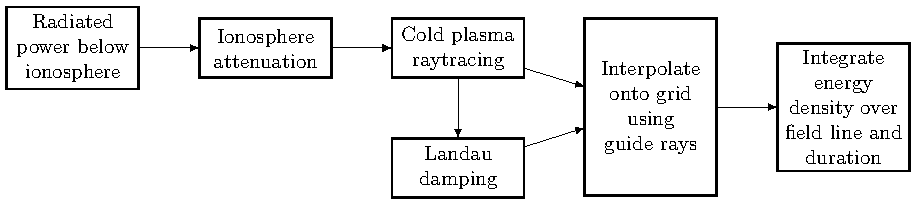
\includegraphics[width=0.8\textwidth]{figures/lightning_power_block_diagram.pdf}
\caption[Energy density calculation block diagram]{Block diagram of the average energy density calculation for a single flash.}
\label{fig:power_blockdiagram}
\end{center}
\end{figure*}


\begin{table}
\caption{Simulation Parameters}
\begin{center}
\begin{tabular}{c|c}
Latitude spacing & 1$^\circ$ \\
Longitude spacing & 1$^\circ$ \\
Frequency range & 200 Hz - 30 kHz \\
Coarse Frequencies & 33 (log-spaced) \\
Fine Frequencies & 20 \\
\hline
ray tracing parameters: & \\
Maximum time & 20 sec \\
Plasmasphere model & Simplified GCPM \\
Magnetic field model & Dipole 
\end{tabular}
\end{center}
\label{tab:simulation_params}
\end{table}%

\subsection{Radiated power above the ionosphere}
Figure \ref{fig:illumination} shows the illumination below the ionosphere resulting from a single 100 kA discharge, as a function of frequency and radial distance. The illumination pattern given in equation \eqref{eqn:farfield_power_fd} is independent of location along the Earth's surface. We multiply this illumination pattern by the absorption model in section \ref{section:trans_ionosphere_atten} to determine illumination above the ionosphere. Figure \ref{fig:illumination} shows example illumination patterns for a set of flash latitudes and MLT.

% Illumination pattern
\begin{figure}[h!]
\begin{center}
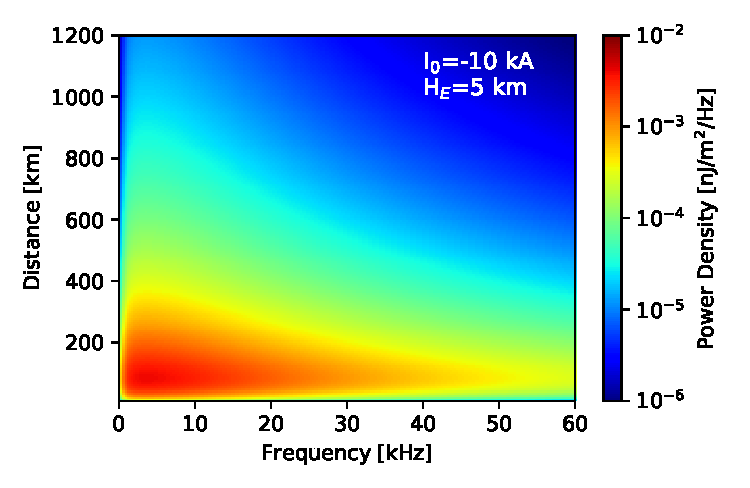
\includegraphics{figures/power_scaling_below_ionosphere.pdf}
\caption[Illumination pattern below the ionosphere]{Vertically-propagating power density below the ionosphere from a single 100kA cloud-to-ground discharge with $H_E=$5 km, as a function of frequency and radial distance. Adapted from \cite{Marshall2011}.}
\label{fig:illumination}
\end{center}
\end{figure}

% Illumination pattern
\begin{figure}
\begin{center}
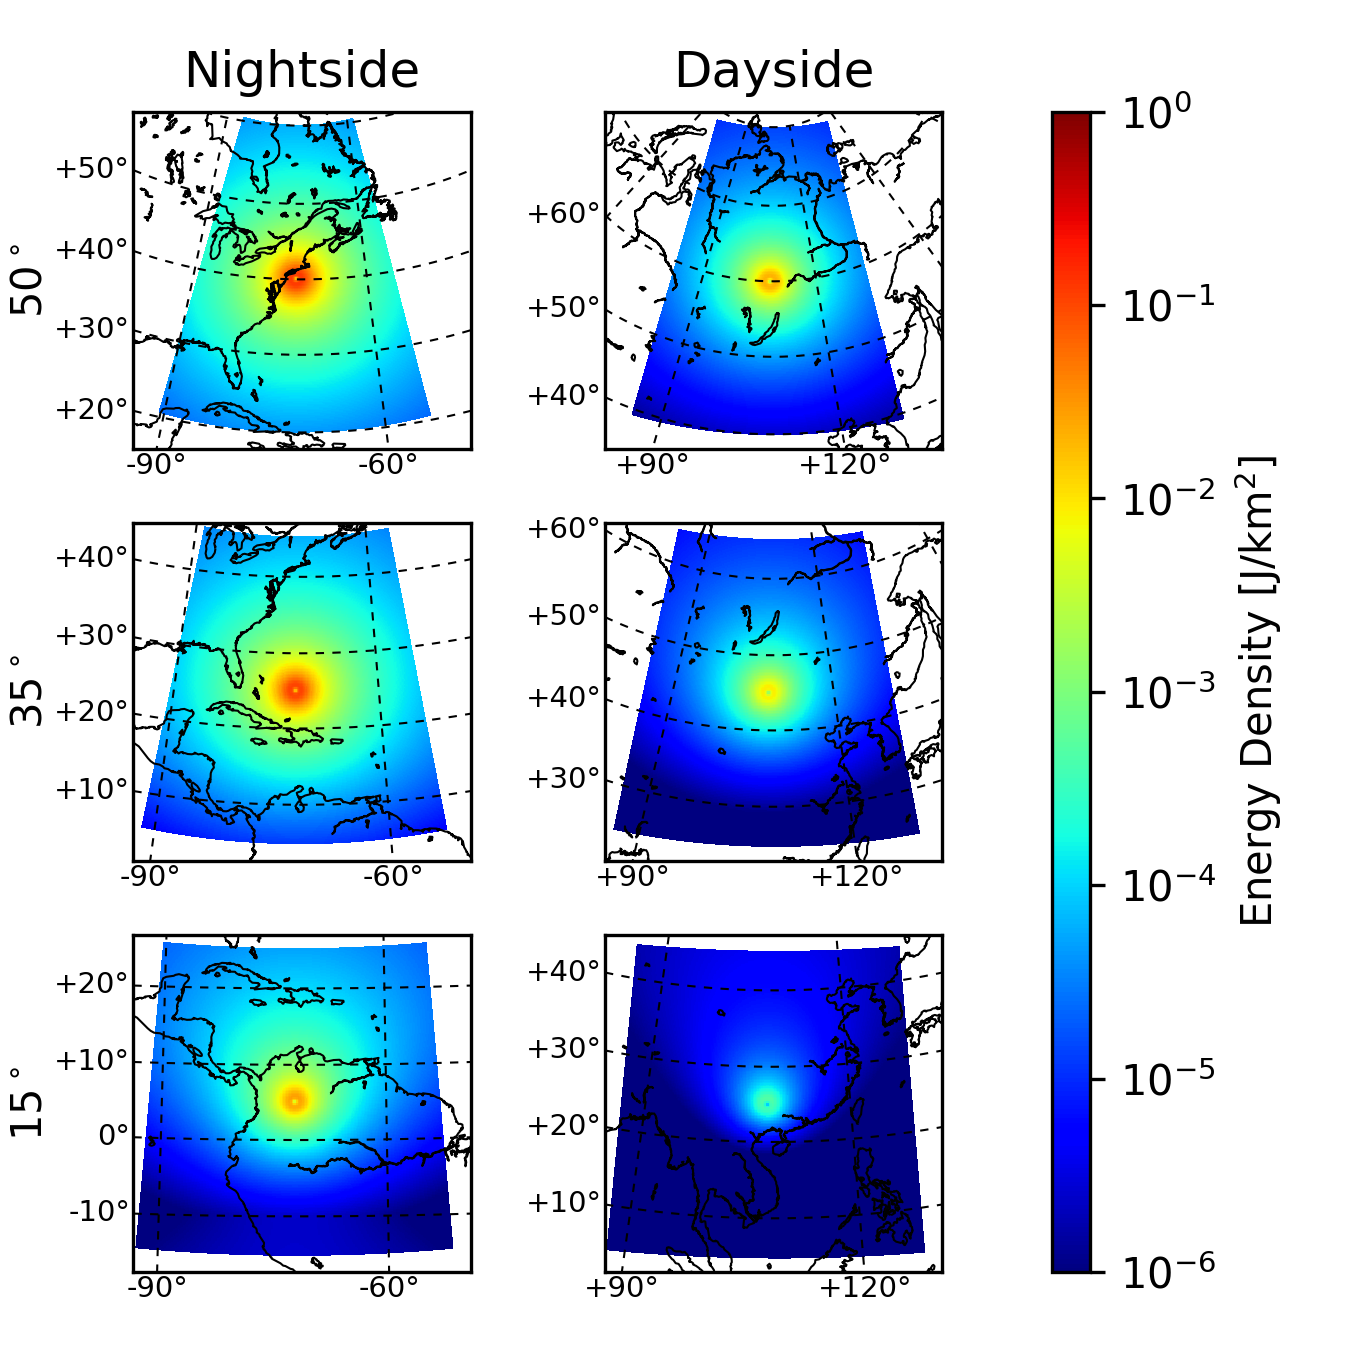
\includegraphics{figures/illumination_basemap.png}
\caption[Illumination pattern above the ionosphere]{Illumination pattern, integrated over frequency, after ionospheric attenuation (altitude = 1000 km).}
\label{fig:illumination}
\end{center}
\end{figure}

% Total energy above ionosphere
\begin{figure}
\begin{center}
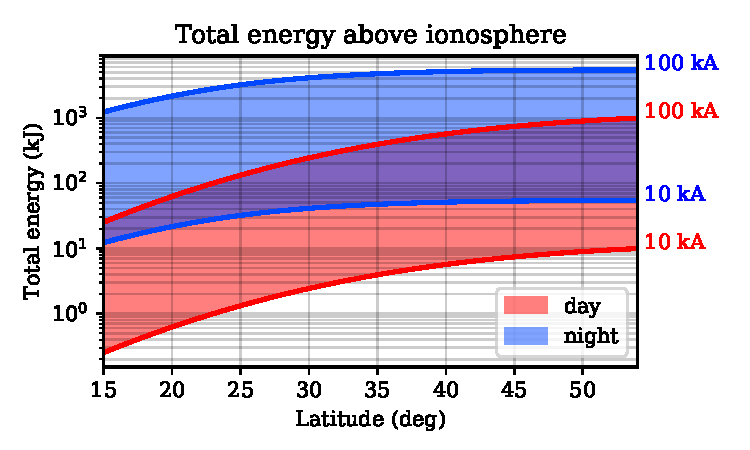
\includegraphics{figures/total_energy.pdf}
\caption[Energy above the ionosphere due to a single flash]{Integrated energy above the ionosphere from a single discharge, as a function of geomagnetic latitude. Energy scales quadratically with peak current; totals for 10 kA (an average flash), and 100 kA (a strong, but not unreasonable flash) are overlaid. The dashed lines indicate the total energy released below the ionosphere, before attenuation.}
\label{fig:illumination_totals}
\end{center}
\end{figure}


\subsection{Gridding and Interpolation}

We now have a model of the total energy above the ionosphere, at an altitude of 1000 km, divided into gridded bins in latitude, longitude, and frequency. The next step required is to map the energy within each cell out into the plasmasphere. We accomplish this task using a ``guide ray'' formulation, as illustrated in figure \ref{fig:interpolation_scheme}.

Using the ray tracing and Landau damping technique from section \ref{section:raytracing}, we compute rays in 1$^\circ$ steps in both latitude and longitude, within 1000 km of the incident flash, for 33 logarithmically-spaced frequencies between 200 Hz and 30 kHz. Rays are computed for 20 seconds. See table \ref{tab:simulation_params} for a list of various parameters used. The computed rays are then interpolated onto a uniform time axis using one-dimensional linear interpolation for each parameter. 

We make the assumption that the energy bounded by the set of 8 guide rays (two latitudes, two longitudes, two frequencies) remains bounded by these rays as they propagate. Furthermore, we assume that our interpolated timesteps are much larger than the envelope of the wave packet (see figure \ref{fig:lightning_spectrum}). Therefore, the initial energy within each cell is bounded by a four-dimensional voxel, determined by two adjacent timesteps $t_{n-1}, t_n$ of the guide ray set \{(lat$_1$, lat$_2$), (lon$_1$, lon$_2$), (f$_1$, f$_2$)\}.

Next, we map the energy within each voxel to our output grid coordinates -- chosen here to be 1$^\circ$ steps in latitude, 0.25$^\circ$ in longitude, and 0.05 L-shell. We accomplish this task using an n-dimensional Delaunay triangulation construction \citep{Delaunay1934, Lee1980}. A Delaunay triangulation breaks the convex hull of a volume, as defined by a set of points in $\mathbb R^n$, into a set of primitive shapes called ``simplexes''. Each simplex is an n-dimensional triangle. 

At each timestep, we compute a Delaunay triangulation for the 16 points defined by corners at \{($t_{n-1}, t_n$), (lat$_1$, lat$_2$), (lon$_1$, lon$_2$), (f$_1$, f$_2$)\}. Once a Delaunay triangulation has been made, it is a computationally-efficient task to check whether or not an arbitrary new point is within any of the simplexes. We use the Scipy Delaunay implementation, which is based on the open-source \emph{qhull} code \citep{Barber1996}. For any point within the volume, we assign to it the average energy density in $J/m^3$ within the voxel at the given timestep, multiplied by the average Landau damping factor. Figure \ref{fig:delaunay_1} illustrates the interpolation method.

\subsubsection{Fine-scale frequency interpolation}
Our output grid coordinates are given in three dimensions -- latitude, longitude, and L-shell. However, our Delaunay construction adds an additional dimension, frequency. We can perform a fine-scale interpolation on the frequency axis by selecting a linearly-spaced grid of sub-frequencies between the two ray frequencies $f_1, f_2$. Checking and logging whether or not each new point is within the four-dimensional voxel is equivalent to interpolating and checking in three dimensions, as illustrated in figure \ref{fig:delaunay_2}.

    \begin{figure}
    \centering
    \begin{subfigure}[t]{0.45\textwidth}
    \centering
        	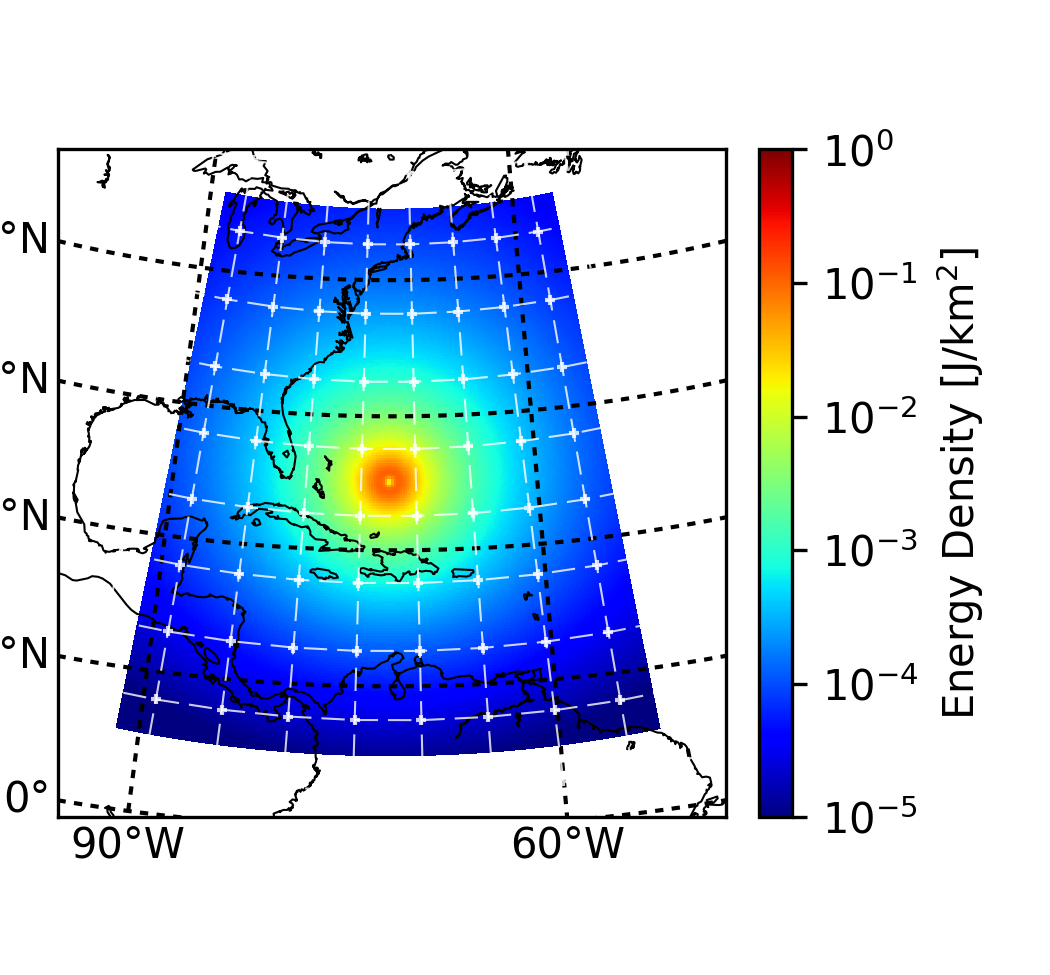
\includegraphics{figures/input_energy_with_grid.png}
	\caption{Input energy gridding}
        \label{fig:input_energy_grid}
    \end{subfigure}\hfill
    \begin{subfigure}[t]{0.45\textwidth}
    \centering
        	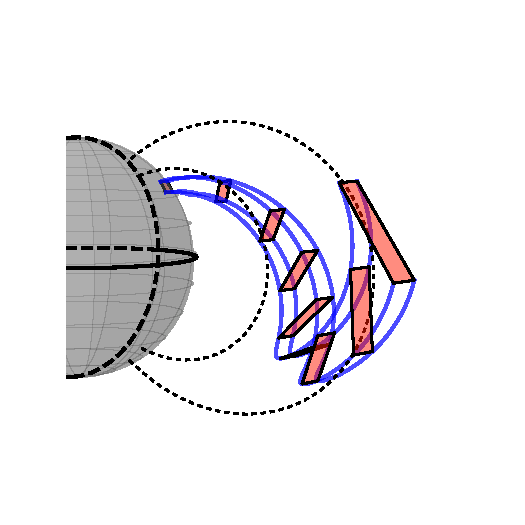
\includegraphics[trim={1cm 0.25cm 1cm 1cm},clip]{figures/interpolation_globe1.pdf}
	\caption{``guide ray'' construction}
        \label{fig:guide_rays}
    \end{subfigure}
    \caption[Illustrations of the interpolation scheme]{An illustration of the interpolation scheme. (a) Energy at the top of the ionosphere is divided into cells, in latitude, longitude, and frequency. Shown here with 5$^\circ$ cells (much larger than used in simulation). The plotted energy is integrated over frequency. (b) Illustration of the guide ray method. Input energy is integrated between a set of guide rays, spaced in latitude, longitude, and frequency. This energy is then averaged over a 4-dimensional volume, bounded by two adjacent timesteps $t_{n-1}$, $t_n$ of the guide rays.}
    \label{fig:interpolation_scheme}
\end{figure}


% Delaunay figure
\begin{figure}
\begin{center}
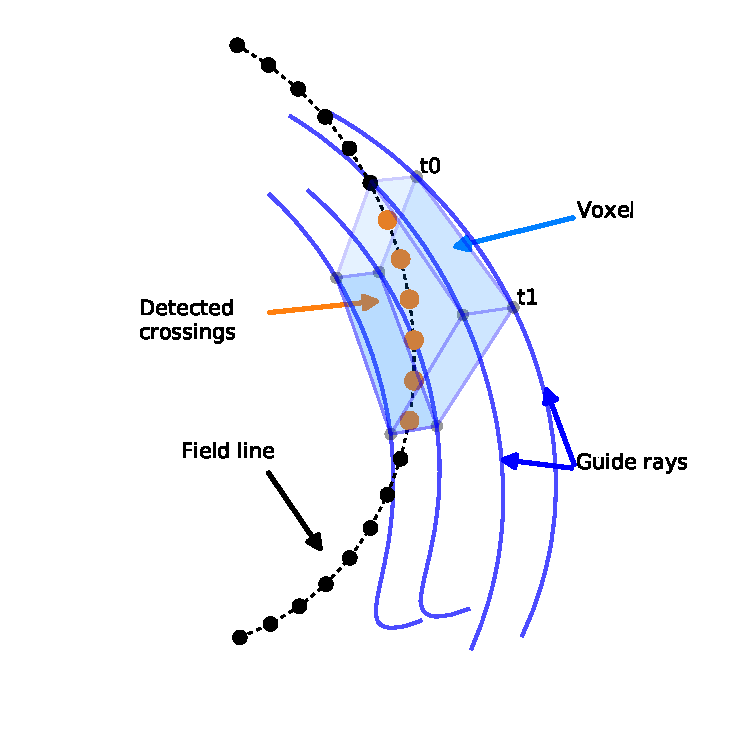
\includegraphics{figures/delaunay_1.pdf}
\caption[Delaunay interpolation method]{Illustration of the Delaunay interpolation method, shown here in three dimensions (e.g., for a single frequency).}
\label{fig:delaunay_1}
\end{center}
\end{figure}

% Fine-scale frequency interpolation
\begin{figure}
\begin{center}
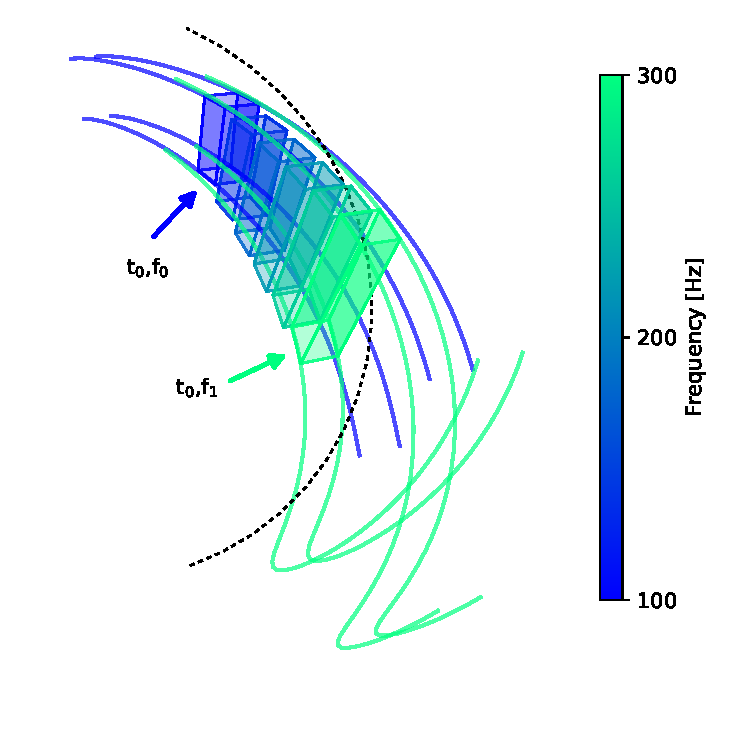
\includegraphics{figures/delaunay_2.pdf}
\caption[Fine-scale frequency interpolation]{An illustration of fine-scale frequency interpolation. Here we show a three-dimensional voxel being linearly interpolated between two sets of guide rays, at $f_1=200$ Hz and $f_2=300$ Hz. Our implementation operates on a four-dimensional voxel, facilitating rapid checking across fine-scale frequency interpolation steps.}
\label{fig:delaunay_2}
\end{center}
\end{figure}

\subsubsection{Discussion}
Our interpolation method differs substantially from \cite{Bortnik2005} and related work. \citeauthor{Bortnik2005} performed an area-weighted interpolation between guide rays in latitude and frequency, and then looked for ray-segment intersections with cross-sectional areas perpendicular to a field line. Crossings, however, are exceedingly rare over the full set of guide rays and output cross-sectional area segments, which requires clever restriction of the output space, or high computational resources. Our method was selected for computational efficiency when relaxing the meridional-plane restriction, and to assure that all input energy is accounted for. Using the \cite{Bortnik2005} method with larger intervals in latitude and longitude can result in undersampling the post-ionosphere illumination pattern, while our method integrates the input energy regardless of grid size.

One caveat of our interpolation algorithm is that the Delaunay triangulation implementation only checks whether or not a point is within the convex hull of the voxel, rather than the voxel itself. For simple voxels, and at early timesteps (e.g., before any magnetospheric reflection), we can be confident that the voxel remains cubic, and the concave and convex hulls are equivalent. However at later timesteps, after the rays have spread and reflected substantially, the concave and convex hulls are likely not equivalent, in which case the interpolation algorithm may artificially disperse the energy over a larger volume, effectively underestimating energy density while overestimating energy spreading. Figure \ref{fig:convex_hulls} shows some simple polygons and their convex hulls.


% CONVEX HULL FIGURE
\begin{figure}
\begin{center}
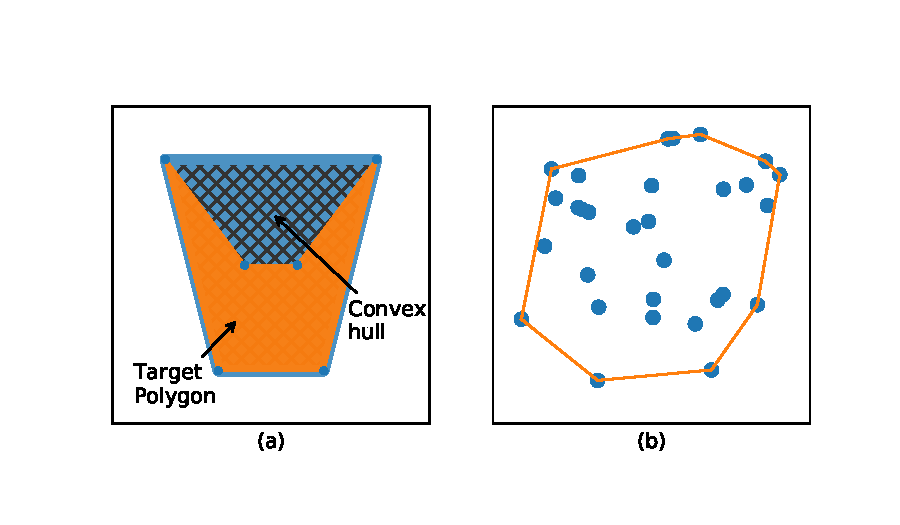
\includegraphics{figures/convex_hulls.pdf}
\caption{Illustration of a convex hull in two dimensions. (a) A simple polygon, shown in orange, for which the convex hull and concave hulls differ substantially. (b) A collection of random points, and their concave hull.}
\label{fig:convex_hulls}
\end{center}
\end{figure}


\subsection{Energy stencils for a single flash}


\begin{figure}
\begin{center}
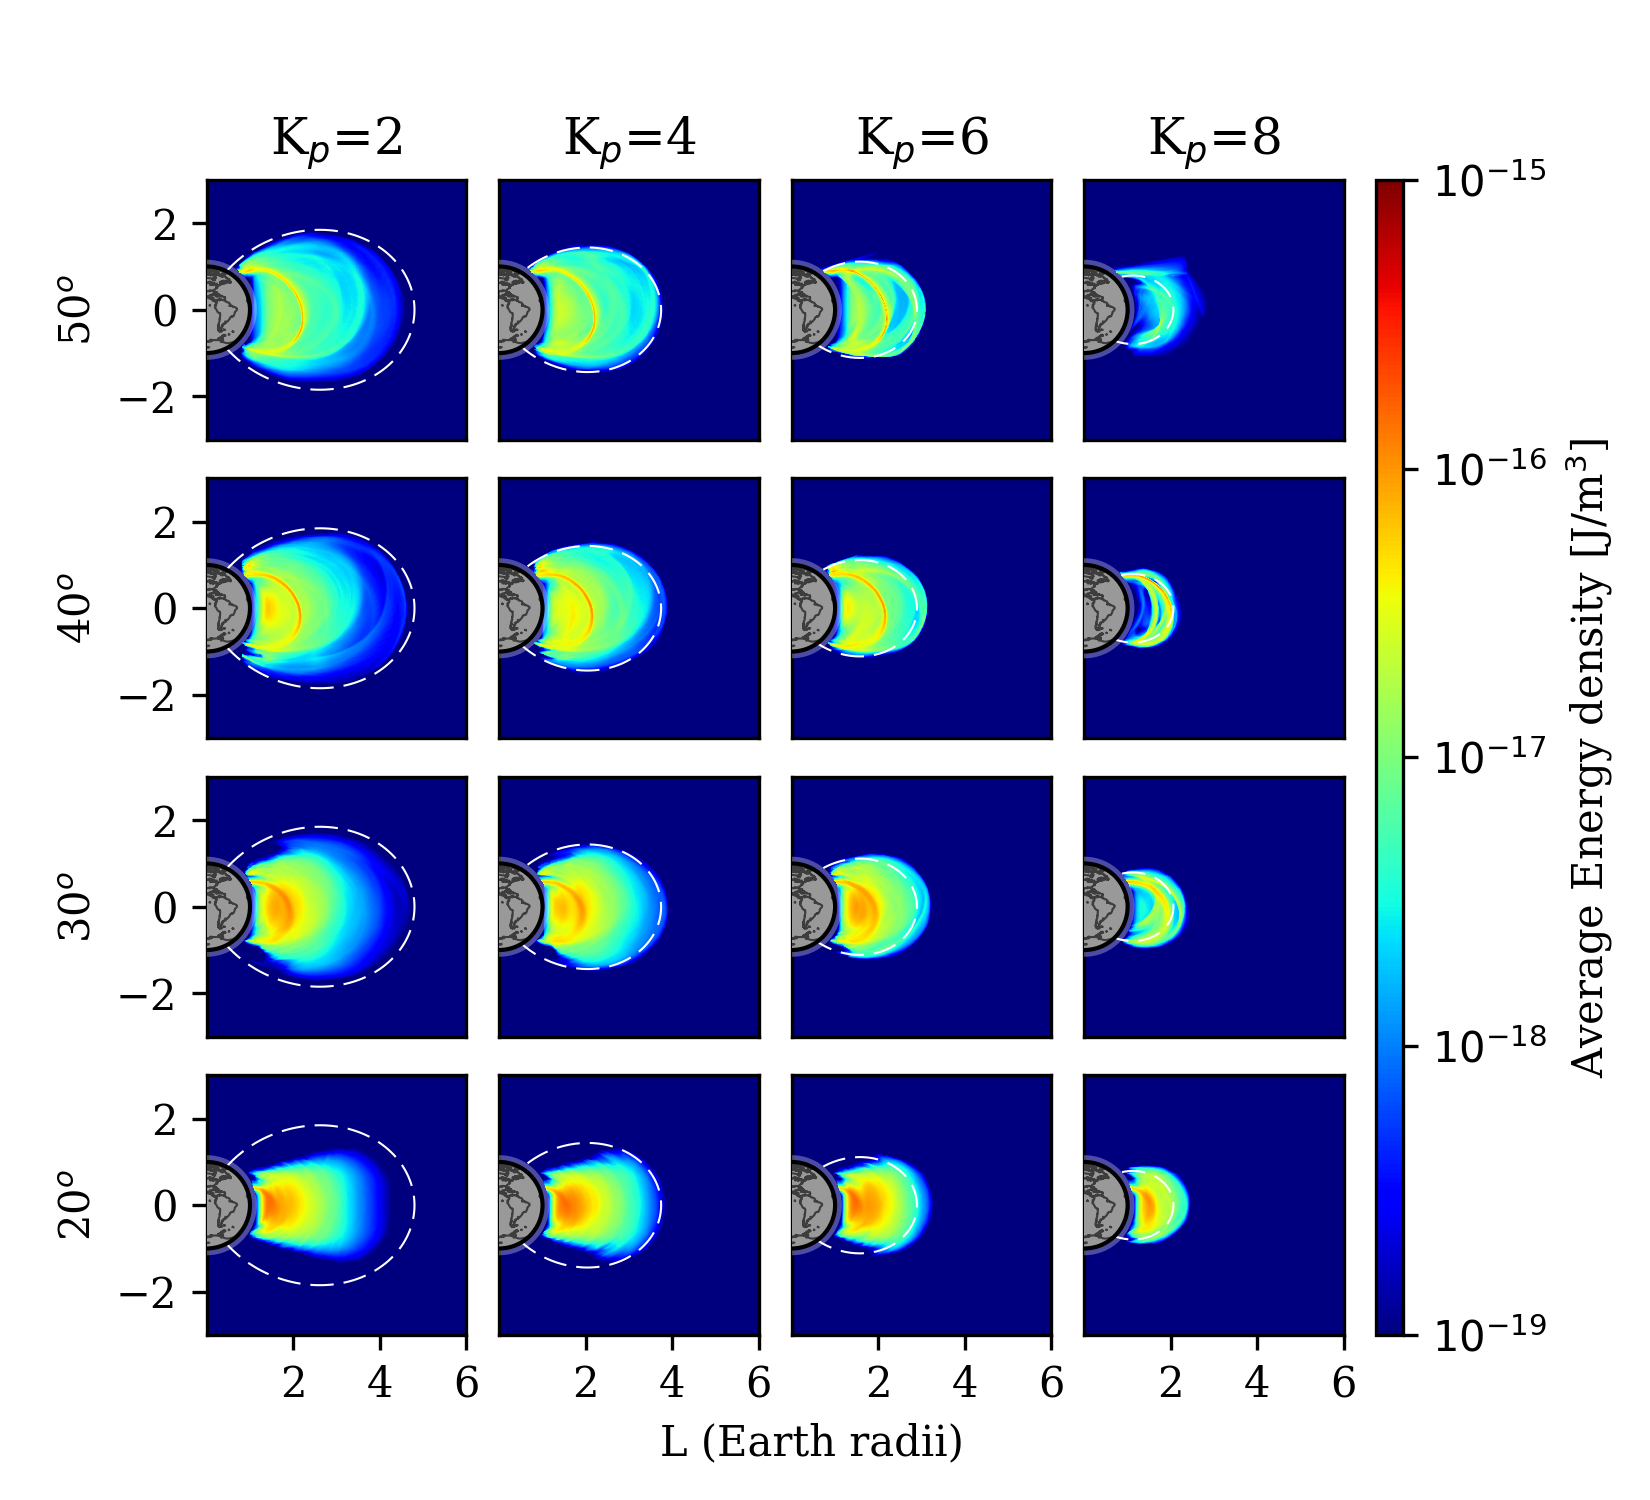
\includegraphics[draft]{figures/energy_from_single_flash_meridonal_plane.pdf}
\caption{Block diagram}
\label{fig:energy_from_single_flash}
\end{center}
\end{figure}

% you'll want to put a figure showing the volume averaging too...

\begin{figure}
\begin{center}
\includegraphics[draft]{figures/energy_in_meridional_plane_movieframes.pdf}
\caption{Block diagram}
\label{fig:energy_from_single_flash}
\end{center}
\end{figure}


\begin{figure}[ht]
\begin{center}
\includegraphics[draft]{figures/energy_stencils.pdf}
\caption{Block diagram}
\label{fig:energy_stencils}
\end{center}
\end{figure}

\section{Global Energy Density}

\begin{figure}
\begin{center}
\includegraphics[draft]{figures/energy_density_vs_L_vs_freq.pdf}
\caption[Average energy density vs L and frequency]{Average energy density as a function of L-shell and wave frequency}
\label{fig:energy_density_vs_L_vs_freq}
\end{center}
\end{figure}
